\section{Risultati}\label{risultati}

\subsection{Tabella dei risultati}
\begin{center}
	\begin{tabularx}{\linewidth}{|c|c|c|c|c|}
		\hline
		{Istanza Soluzione} & {Tempo(s)} & \parbox{3cm}{\vspace{.1cm}\centering Tempo Full Contraction(s)\vspace{.1cm}} & {Discovery time(s)} & {Errore(\%)}\\\hline
		input\_random\_8\_10.txt&&&&
	\end{tabularx}
\end{center}

%\subsection{Grafico di confronto dei tempi di esecuzione}
%\begin{center}
%	\begin{figure}[H]
%		\centering
%		\hspace{-1cm}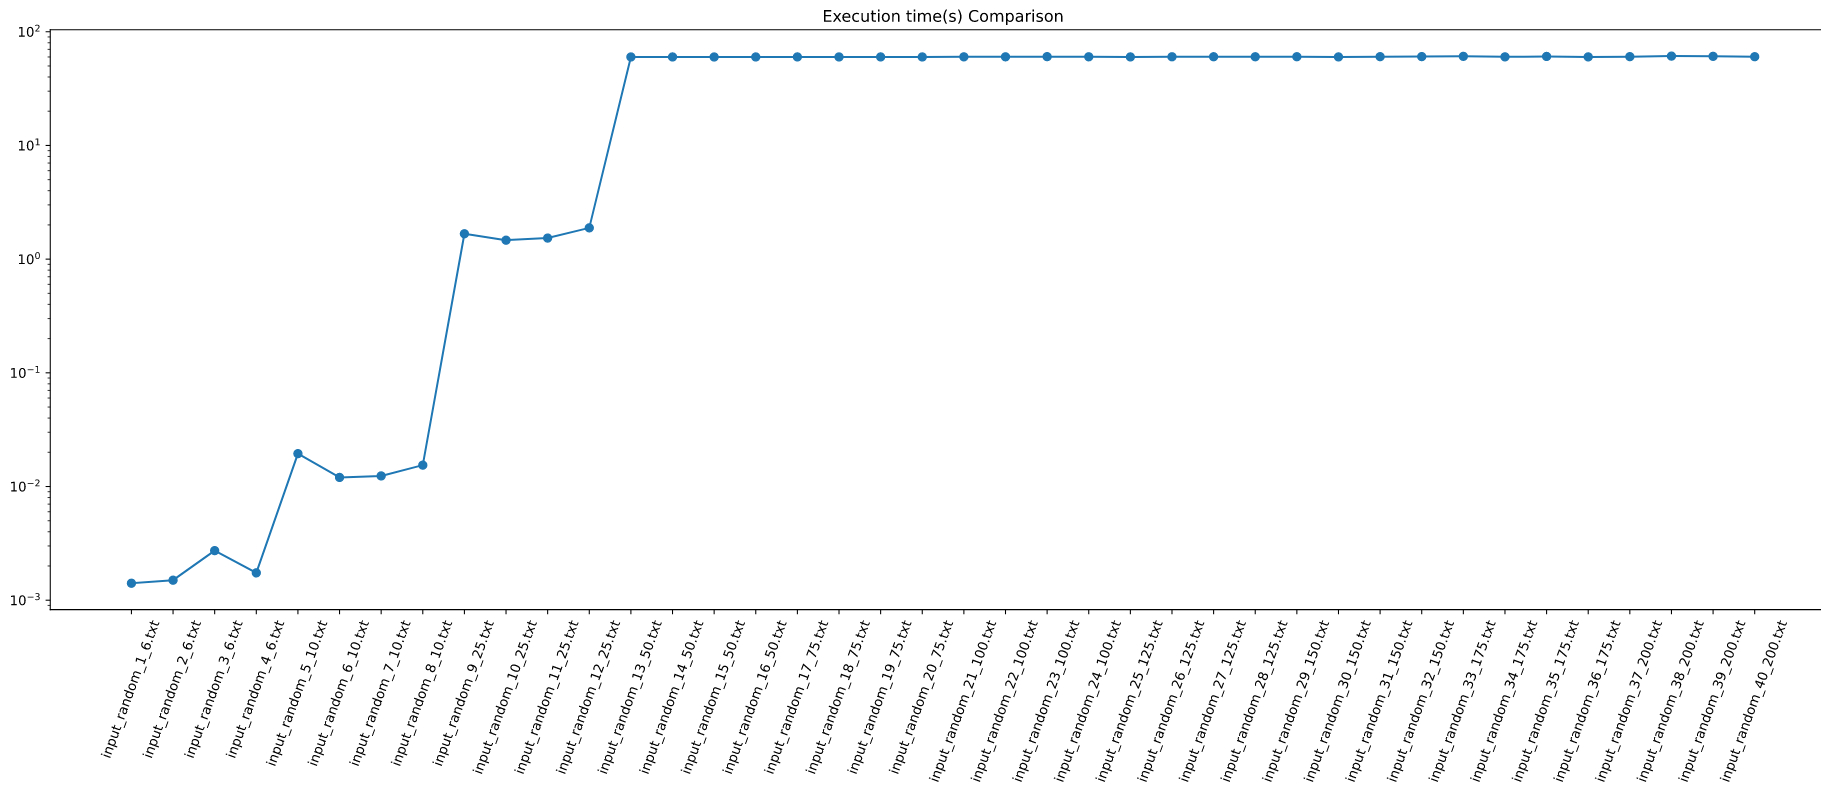
\includegraphics[width=12cm]{Img/exec_time_graph.jpg}
%		\caption{Confronto dei tempi di esecuzione}
%	\end{figure}
%\end{center}
%
%\subsection{Grafico di confronto dei tempi di Full Contraption}
%\begin{center}
%	\begin{figure}[H]
%		\centering
%		\hspace{-1cm}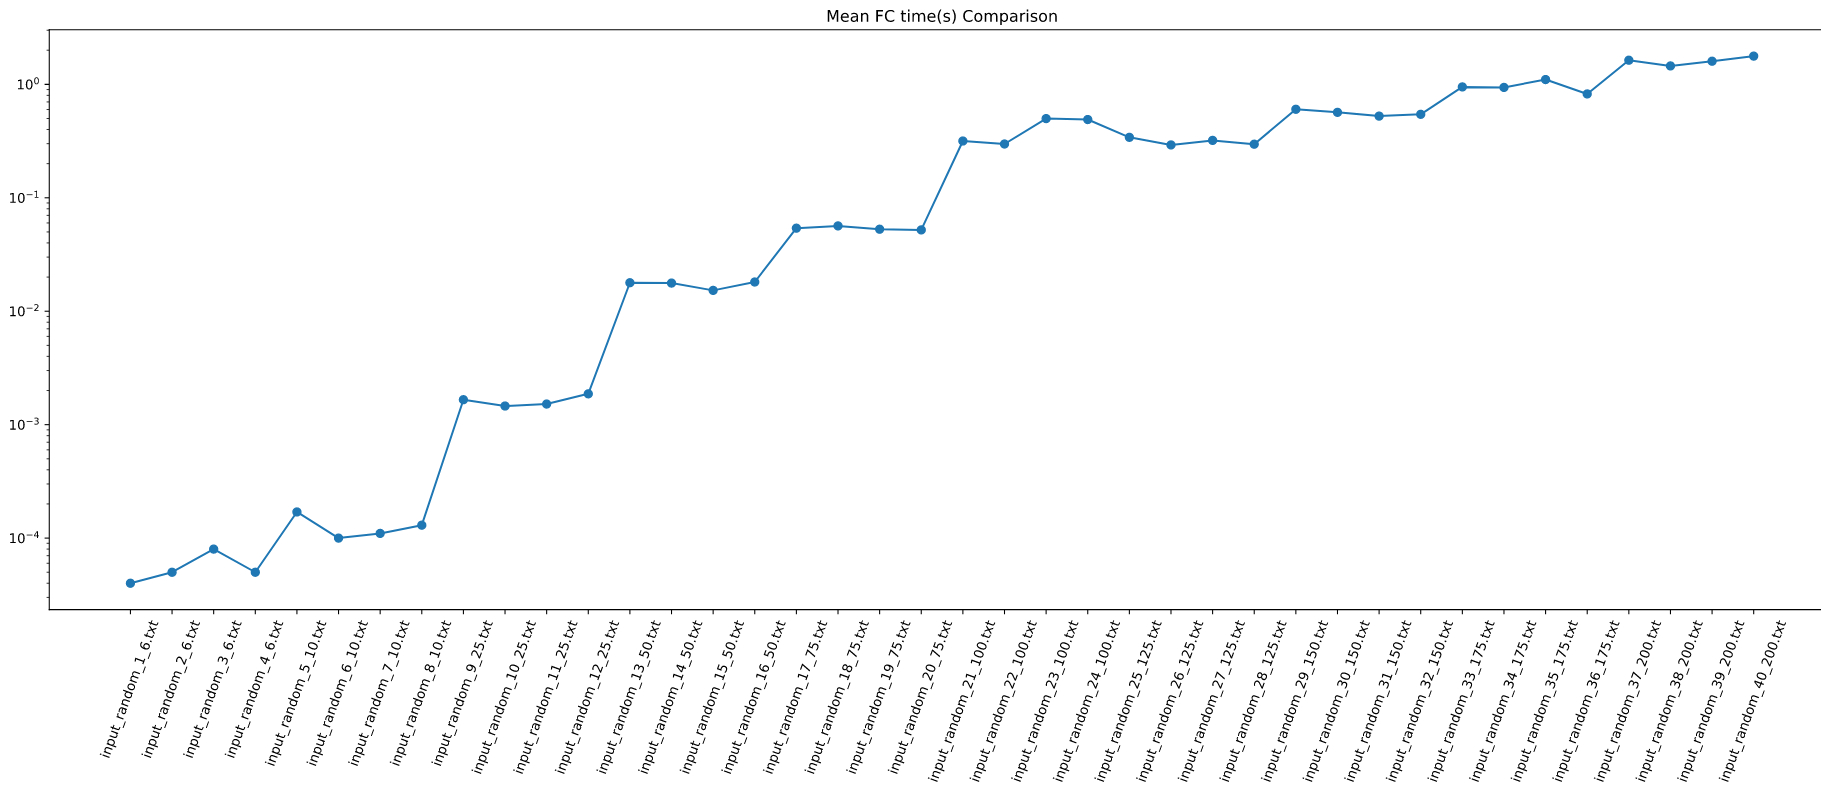
\includegraphics[width=12cm]{Img/fc_time_graph.jpg}
%		\caption{Confronto dei tempi di Full Contraption}
%	\end{figure}
%\end{center}
%
%\subsection{Grafico di confronto dei Discovery Time}
%\begin{center}
%	\begin{figure}[H]
%		\centering
%		\hspace{-1cm}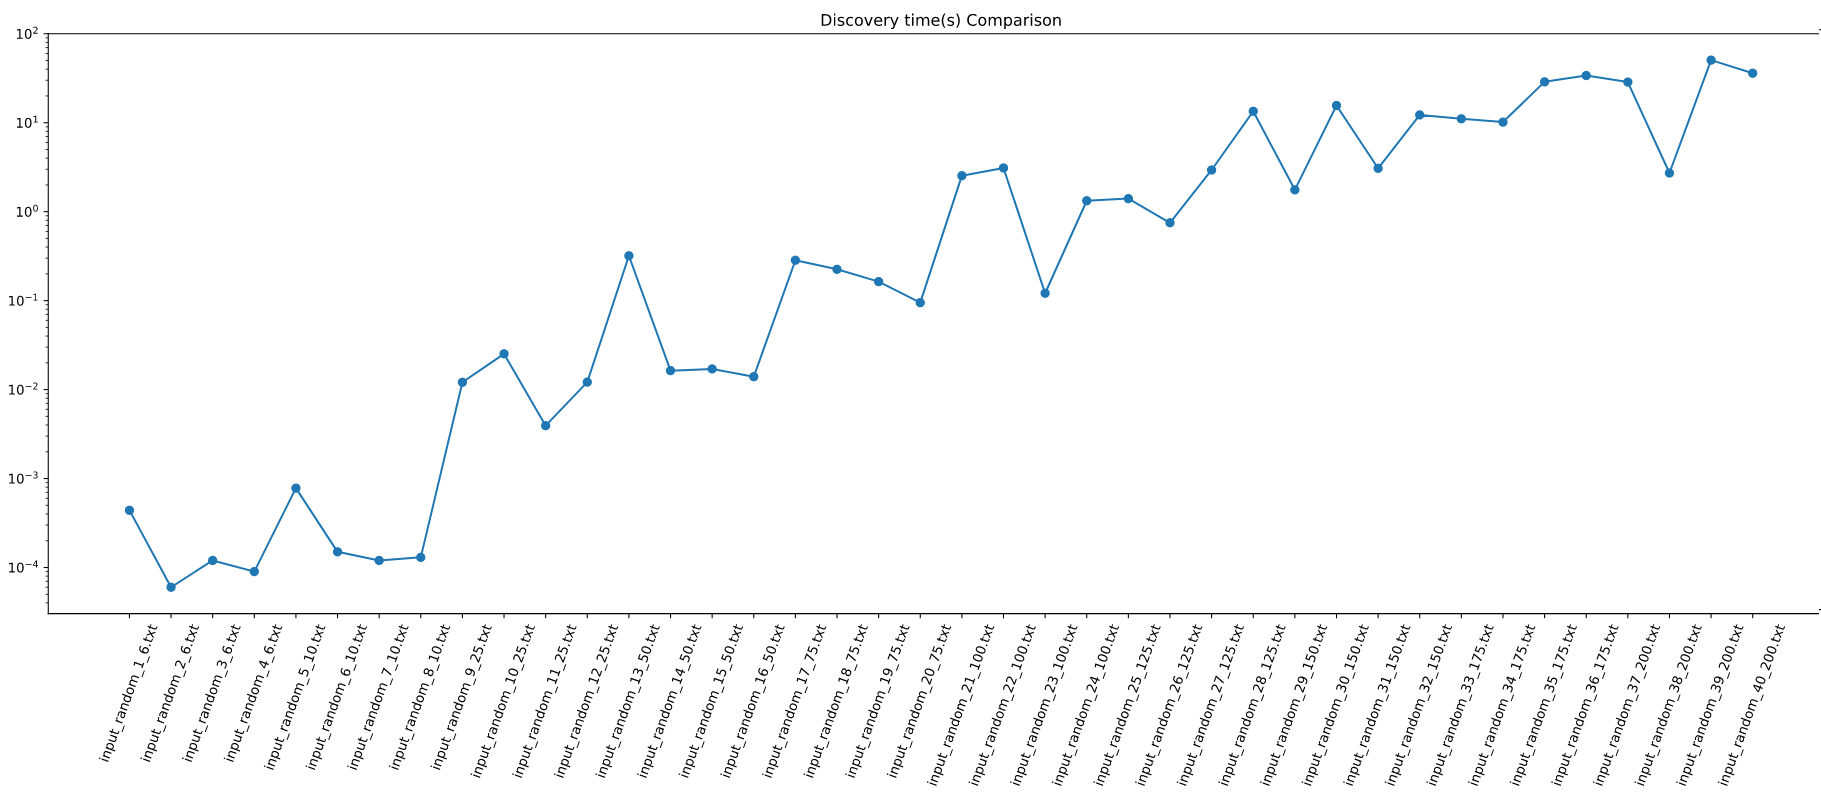
\includegraphics[width=16cm]{Img/disc_time_graph.jpg}
%		\caption{Confronto dei Discovery Time}
%	\end{figure}
%\end{center}
%
%\subsection{Grafico di confronto delle percentuali di errore}
%\begin{center}
%	\begin{figure}[H]
%		\centering
%		\hspace{-1cm}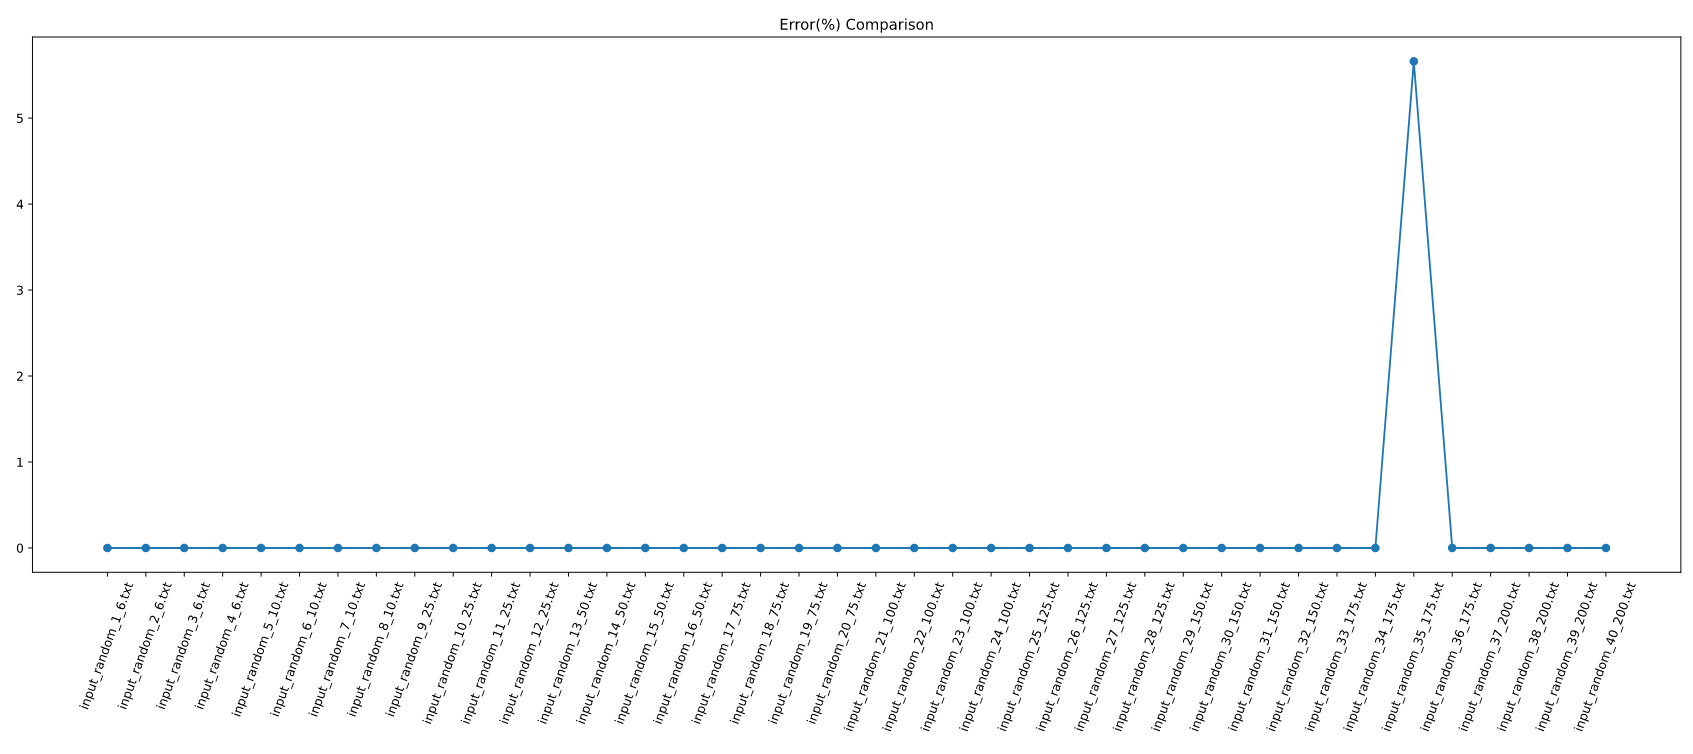
\includegraphics[width=16cm]{Img/err_perc_graph.jpg}
%		\caption{Confronto delle percentuali di errore}
%	\end{figure}
%\end{center}

\pagebreak